\section*{Синтез недвоичного вычитающего счетчика}
\addcontentsline{toc}{section}{Синтез недвоичного вычитающего счетчика}

\subsection*{Построение аналитической модели}
\addcontentsline{toc}{subsection}{Построение аналитической модели}

Исходя из условия необходимо построить недвоичный вычитающий счетчик с $K_{\text{СЧ}}=5$. 
Первоначально определим количество триггеров необходимых для построения. Для расчета
воспользуемся следующим соотношением:

$$
    m \geq \left| \log_{2}{M} \right| \approx 2.32 \Rightarrow m=3
$$

Далее производем рассчет избыточных состояний счетчика:

$$
    N=2^m - K_{\underset{n}{\sim}} = 8 - 5 = 3
$$

Имеем 3 избыточных состояния, которые необходимо исключить из возможных состояний счетчика. 
Исключим следующие состояния: $\overline{Q_1} \ \overline{Q_2} \ \overline{Q_3}, \
Q_1 \overline{Q_2} \ \overline{Q_3},\ \overline{Q_1} Q_2 \overline{Q_3}$. \par

Затем необходимо определить порядок изменения состояний счетчика. При состовление порядка необходимо
учесть, что необходимо построить \textit{вычитающий} счетчик, а значит номер каждого последующего состояние
должнен быть на единицу меньше предшествующего. Имеем итоговый порядок состояний:

$$
    Q_1 Q_2 Q_3 \rightarrow
    \overline{Q_1} Q_2 Q_3 \rightarrow
    Q_1 \overline{Q_2} Q_3 \rightarrow
    \overline{Q_1} \ \overline{Q_2} Q_3 \rightarrow
    Q_1 Q_2 \overline{Q_3} \rightarrow
    Q_1 Q_2 Q_3 \rightarrow \dots
$$

На основании построенного порядка переходов состояния счетка построим таблицу функционирования:

\begin{table}[h!]
    \begin{center}
        \begin{tabular}{
            |>\centering m{0.35cm}
            |>\centering m{1cm}
            |>\centering m{1cm}
            |>\centering m{1cm}
            |>\centering m{1cm}
            |>\centering m{1cm}
            |>{\centering\arraybackslash} m{1cm} |
        }
            \hline
             &  &  &  &  &  &  \\[-4mm]
            № & $Q_1^t$ & $Q_2^t$ & $Q_3^t$ & $Q_1^{t+1}$ & $Q_2^{t+1}$ & $Q_3^{t+1}$ \\ \hline \hline
            0 & 1 & 1 & 1 & 0 & 1 & 1 \\ \hline
            1 & 0 & 1 & 1 & 1 & 0 & 1 \\ \hline
            2 & 1 & 0 & 1 & 0 & 0 & 1 \\ \hline
            3 & 0 & 0 & 1 & 1 & 1 & 0 \\ \hline
            4 & 1 & 1 & 0 & 1 & 1 & 1 \\ \hline
        \end{tabular}
        \caption{Таблица функционирования счетчика}
        \label{table:1}
    \end{center}
\end{table}

На основании таблицы функционирования счетчика были составлены прикладные таблицы для каждого триггера счетчика. 
Данные таблицы отражают переход конкретного триггера из предыдущего состояния в следующее. В составленных таблицах,
в клетках пересечения указаны двоичные числа, отражающие переход триггера при изменении состояния автомата.
Пустые клетки соответвуют исключенным состояниям. \par

\begin{center}
    \begin{tabular}{
        |>\centering m{2cm}
        |>\centering m{1cm}
        |>\centering m{1cm}
        |>\centering m{1cm}
        |>{\centering\arraybackslash} m{1cm} |
    }
        \hline
        &  &  &  & \\[-4mm]
        $Q_1^t \rightarrow Q_1^{t+1}$ & $Q_2$ & $Q_2$ & $\overline{Q_2}$ & $\overline{Q_2}$ \\ \hline
        &  &  &  & \\[-4mm]
        $Q_3$ & 01 & 10 & 10 & 01 \\ \hline
        &  &  &  & \\[-4mm]
        $\overline{Q_3}$ & - & 11 & - & - \\ \hline
        &  &  &  & \\[-4mm]
        & $\overline{Q_1}$ & $Q_1$ & $Q_1$ & $\overline{Q_1}$ \\ 
        \hline
    \end{tabular}
    \captionof{table}{Прикладная таблица $Q_1$}
    \label{table:2}

    \newpage

    \begin{tabular}{
        |>\centering m{2cm}
        |>\centering m{1cm}
        |>\centering m{1cm}
        |>\centering m{1cm}
        |>{\centering\arraybackslash} m{1cm} |
    }
        \hline
        &  &  &  & \\[-4mm]
        $Q_2^t \rightarrow Q_2^{t+1}$ & $Q_2$ & $Q_2$ & $\overline{Q_2}$ & $\overline{Q_2}$ \\ \hline
        &  &  &  & \\[-4mm]
        $Q_3$ & 10 & 11 & 00 & 01 \\ \hline
        &  &  &  & \\[-4mm]
        $\overline{Q_3}$ & - & 11 & - & - \\ \hline
        &  &  &  & \\[-4mm]
        & $\overline{Q_1}$ & $Q_1$ & $Q_1$ & $\overline{Q_1}$ \\ 
        \hline
    \end{tabular}
    \captionof{table}{Прикладная таблица $Q_2$}
    \label{table:3}

    \vspace*{5mm}

    \begin{tabular}{
        |>\centering m{2cm}
        |>\centering m{1cm}
        |>\centering m{1cm}
        |>\centering m{1cm}
        |>{\centering\arraybackslash} m{1cm} |
    }
        \hline
        &  &  &  & \\[-4mm]
        $Q_3^t \rightarrow Q_3^{t+1}$ & $Q_2$ & $Q_2$ & $\overline{Q_2}$ & $\overline{Q_2}$ \\ \hline
        &  &  &  & \\[-4mm]
        $Q_3$ & 11 & 11 & 11 & 10 \\ \hline
        &  &  &  & \\[-4mm]
        $\overline{Q_3}$ & - & 01 & - & - \\ \hline
        &  &  &  & \\[-4mm]
        & $\overline{Q_1}$ & $Q_1$ & $Q_1$ & $\overline{Q_1}$ \\ 
        \hline
    \end{tabular}
    \captionof{table}{Прикладная таблица $Q_3$}
    \label{table:4}
\end{center}

В качестве элементной базы выберем триггеры J-K типа K155ТВ1, в виду их универсальности. 
Характеристическая таблица J-K триггера:

\begin{center}
    \begin{tabular}{
        |>\centering m{2cm}
        |>\centering m{1cm}
        |>{\centering\arraybackslash} m{1cm} |
    }
        \hline
        & & \\[-4mm]
        $Q^t \rightarrow Q^{t+1}$ & $J^t$ & $K^t$ \\ \hline
        00 & 0 & * \\ \hline
        01 & 1 & * \\ \hline
        10 & * & 1 \\ \hline
        11 & * & 0 \\ \hline
    \end{tabular}
    \captionof{table}{Характеристическая таблица для J-K-триггера}
    \label{table:5}
\end{center}

Опираясь на характеристическую таблицу триггера построим карты Карно для J и K входов заменив 
двоичные значения на пересечениях соответствующими значениями из характерестической таблицы. \par

\begin{center}
    \begin{minipage}[l]{65mm}
        \begin{tabular}{
            |>\centering m{0.6cm}
            |>\centering m{0.9cm}
            |>\centering m{0.9cm}
            |>\centering m{0.9cm}
            |>{\centering\arraybackslash} m{0.9cm} |
        }
            \hline
            &&&& \\[-4mm]
            $J_1$ & $Q_2$ & $Q_2$ & $\overline{Q_2}$ & $\overline{Q_2}$ \rowend
            &&&& \\[-4mm]
            $Q_3$ & 1 & * & * & 1 \rowend
            &&&& \\[-4mm]
            $\overline{Q_3}$ & - & * & - & - \rowend
            &&&& \\[-4mm]
            & $\overline{Q_1}$ & $Q_1$ & $Q_1$ & $\overline{Q_1}$ \rowend
        \end{tabular}
        \captionof{table}{Карта Карно для $J_1$}
    \end{minipage}
    \hspace{10mm}
    \begin{minipage}[l]{65mm}
        \begin{tabular}{
            |>\centering m{0.6cm}
            |>\centering m{0.9cm}
            |>\centering m{0.9cm}
            |>\centering m{0.9cm}
            |>{\centering\arraybackslash} m{0.9cm} |
        }
            \hline
            &&&& \\[-4mm]
            $K_1$ & $Q_2$ & $Q_2$ & $\overline{Q_2}$ & $\overline{Q_2}$ \rowend
            &&&& \\[-4mm]
            $Q_3$ & * & 1 & 1 & * \rowend
            &&&& \\[-4mm]
            $\overline{Q_3}$ & - & 0 & - & - \rowend
            &&&& \\[-4mm]
            & $\overline{Q_1}$ & $Q_1$ & $Q_1$ & $\overline{Q_1}$ \rowend
        \end{tabular}
        \captionof{table}{Карта Карно для $K_1$}
    \end{minipage}

    \begin{minipage}[l]{65mm}
        \begin{tabular}{
            |>\centering m{0.6cm}
            |>\centering m{0.9cm}
            |>\centering m{0.9cm}
            |>\centering m{0.9cm}
            |>{\centering\arraybackslash} m{0.9cm} |
        }
            \hline
            &&&& \\[-4mm]
            $J_2$ & $Q_2$ & $Q_2$ & $\overline{Q_2}$ & $\overline{Q_2}$ \rowend
            &&&& \\[-4mm]
            $Q_3$ & * & * & 0 & 1 \rowend
            &&&& \\[-4mm]
            $\overline{Q_3}$ & - & * & - & - \rowend
            &&&& \\[-4mm]
            & $\overline{Q_1}$ & $Q_1$ & $Q_1$ & $\overline{Q_1}$ \rowend
        \end{tabular}
        \captionof{table}{Карта Карно для $J_2$}
    \end{minipage}
    \hspace{10mm}
    \begin{minipage}[l]{65mm}
        \begin{tabular}{
            |>\centering m{0.6cm}
            |>\centering m{0.9cm}
            |>\centering m{0.9cm}
            |>\centering m{0.9cm}
            |>{\centering\arraybackslash} m{0.9cm} |
        }
            \hline
            &&&& \\[-4mm]
            $K_2$ & $Q_2$ & $Q_2$ & $\overline{Q_2}$ & $\overline{Q_2}$ \rowend
            &&&& \\[-4mm]
            $Q_3$ & 1 & 0 & * & * \rowend
            &&&& \\[-4mm]
            $\overline{Q_3}$ & - & 0 & - & - \rowend
            &&&& \\[-4mm]
            & $\overline{Q_1}$ & $Q_1$ & $Q_1$ & $\overline{Q_1}$ \rowend
        \end{tabular}
        \captionof{table}{Карта Карно для $K_2$}
    \end{minipage}
    
    \begin{minipage}[l]{65mm}
        \begin{tabular}{
            |>\centering m{0.6cm}
            |>\centering m{0.9cm}
            |>\centering m{0.9cm}
            |>\centering m{0.9cm}
            |>{\centering\arraybackslash} m{0.9cm} |
        }
            \hline
            &&&& \\[-4mm]
            $J_3$ & $Q_2$ & $Q_2$ & $\overline{Q_2}$ & $\overline{Q_2}$ \rowend
            &&&& \\[-4mm]
            $Q_3$ & * & * & * & * \rowend
            &&&& \\[-4mm]
            $\overline{Q_3}$ & - & 1 & - & - \rowend
            &&&& \\[-4mm]
            & $\overline{Q_1}$ & $Q_1$ & $Q_1$ & $\overline{Q_1}$ \rowend
        \end{tabular}
        \captionof{table}{Карта Карно для $J_3$}
    \end{minipage}
    \hspace{10mm}
    \begin{minipage}[l]{65mm}
        \begin{tabular}{
            |>\centering m{0.6cm}
            |>\centering m{0.9cm}
            |>\centering m{0.9cm}
            |>\centering m{0.9cm}
            |>{\centering\arraybackslash} m{0.9cm} |
        }
            \hline
            &&&& \\[-4mm]
            $K_3$ & $Q_2$ & $Q_2$ & $\overline{Q_2}$ & $\overline{Q_2}$ \rowend
            &&&& \\[-4mm]
            $Q_3$ & 0 & 0 & 0 & 1 \rowend
            &&&& \\[-4mm]
            $\overline{Q_3}$ & - & * & - & - \rowend
            &&&& \\[-4mm]
            & $\overline{Q_1}$ & $Q_1$ & $Q_1$ & $\overline{Q_1}$ \rowend
        \end{tabular}
        \captionof{table}{Карта Карно для $K_3$}
    \end{minipage}
\end{center}
\newpage

Ниже приведены полученные логические функции входов всех трех тригеров:

\begin{center}
    \begin{tabular}{
        m{3cm}
        m{3cm}
    }
        $J_1^t=1$ & $K_1^t=Q_3$ \\[5mm]
        $J_2^t=\overline{Q}_1$ & $K_2^t=\overline{Q}_1$ \\[5mm]
        $J_3^t=1$ & $K_3^t=\overline{Q}_1 \ \overline{Q}_2$ \\
    \end{tabular}
\end{center}

При построение логических функций было учтено, что в клетках с $*$ функция неопределенна,
а значит данные клетки можно интерпретировать по своему усмотрению. \par

\subsection*{Построение счетчика в Multisim}
\addcontentsline{toc}{subsection}{Построение счетчика в Multisim}

На основание составленных ранее логических функций входов составим модель (рис. \ref{image:1}).

\begin{figure}[h]
    \centering
    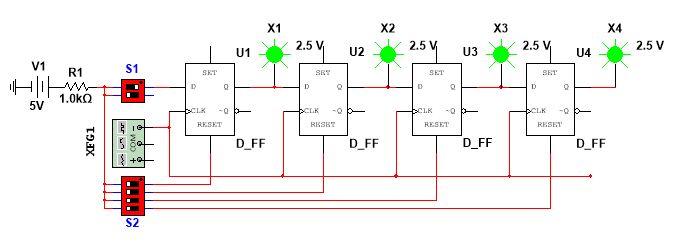
\includegraphics[scale=0.7]{image-1.png}
    \caption{Модель счетчика}
    \label{image:1}
\end{figure}

Протестируем составленную схему. Для проверки будем последовательно подавать входные сигналы на триггеры,
на выходе ожидаем последовательное переключение индикатора OUT ($Q_1Q_2Q_3$ сверху-вниз) в соответвие с порядком

$$
    Q_1 Q_2 Q_3 \rightarrow
    \overline{Q_1} Q_2 Q_3 \rightarrow
    Q_1 \overline{Q_2} Q_3 \rightarrow
    \overline{Q_1} \ \overline{Q_2} Q_3 \rightarrow
    Q_1 Q_2 \overline{Q_3} \rightarrow
    Q_1 Q_2 Q_3 \rightarrow \dots
$$


\begin{center}
    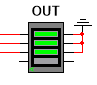
\includegraphics[width=.1\textwidth]{images/image-2.png}\hfill
    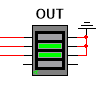
\includegraphics[width=.1\textwidth]{images/image-3.png}\hfill
    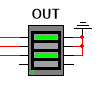
\includegraphics[width=.1\textwidth]{images/image-4.png}\hfill
    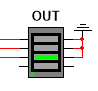
\includegraphics[width=.1\textwidth]{images/image-5.png}\hfill
    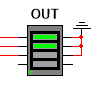
\includegraphics[width=.1\textwidth]{images/image-6.png}\hfill
    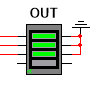
\includegraphics[width=.1\textwidth]{images/image-7.png}
\end{center}

Результат соответвует ожиданию.